\section{SaUCy}
\label{sec:saucy}

Using ILC, we build a concrete, executable implementation of the UC framework,
dubbed SaUCy. Then, we demonstrate the versatility of SaUCy in three ways:
\begin{enumerate}[leftmargin=*]
\item We define a protocol composition operator and its associated composition theorem.
\item We walk through an instantiation of UC commitments.
\item We use ILC's type system to reason about ``reentrancy,'' a subtle definitional issue in UC that has only recently been studied.
\end{enumerate}


%\begin{figure}
%  \centering
%  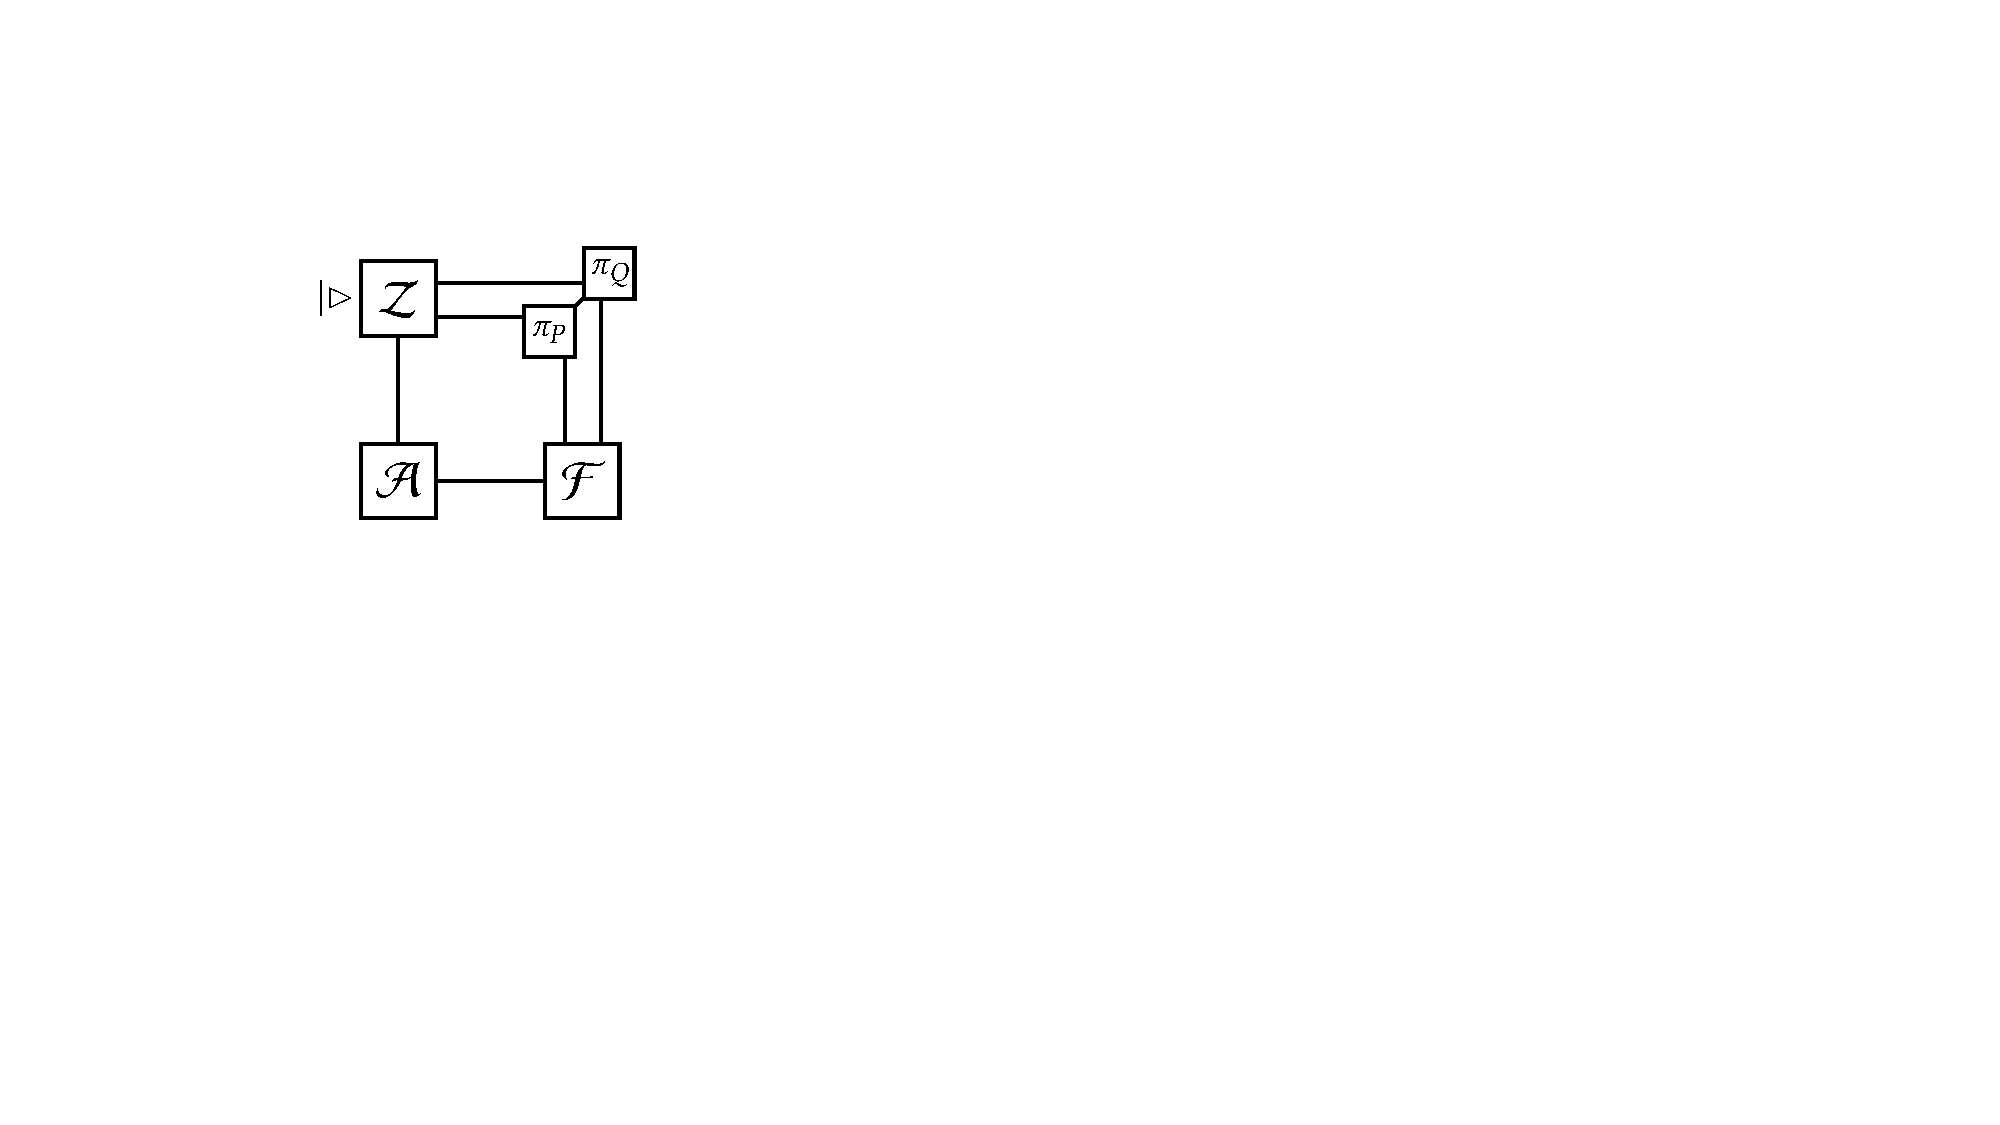
\includegraphics[width=0.4\linewidth]{graphics/execUC}
%  \caption{UC execution.}
%  \label{fig:execUC}
%\end{figure}

\subsection{The UC Framework, Concretely}
\label{subsec:concrete-uc}

\setlength\intextsep{0pt}
\setlength{\columnsep}{10pt}
\begin{wrapfigure}{R}{0.15\textwidth}
\centering
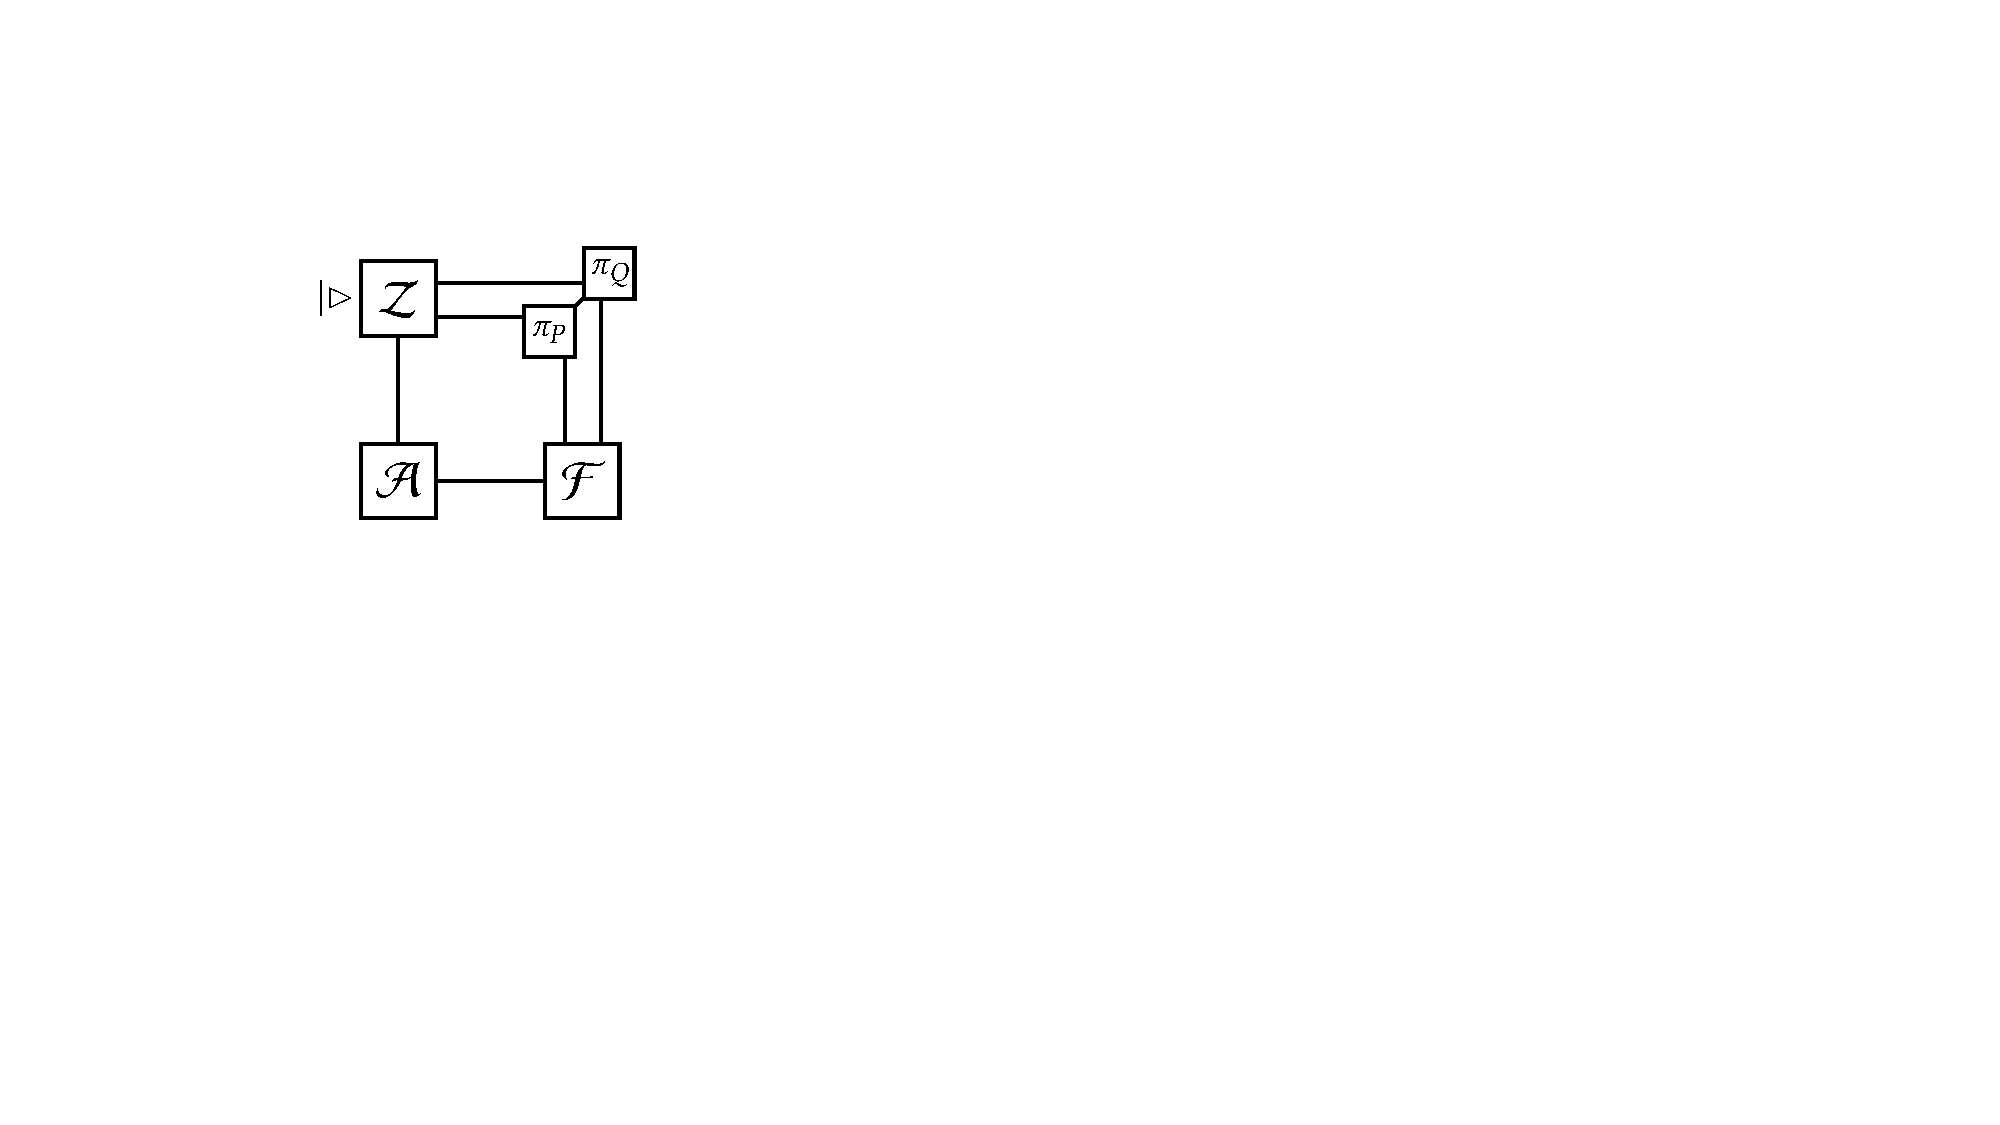
\includegraphics[width=0.15\textwidth]{graphics/execUC}
\caption{\textsf{execUC}.}
\label{fig:execUC-diagram}
\end{wrapfigure}
The first challenge in SaUCy is to define the UC execution model in ILC.  In
principle, this is simple and routes messages as illustrated in
Figure~\ref{fig:execUC-diagram} to the right. For demonstration, we only show
the case of two-party protocols (\`{a} la Simplified
UC~\cite{canetti2015simpler}), which will suffice for our example of
instantiating universally composable commitments.  Also, we will only aim to
show the case of \emph{static} corruptions, in which parties are corrupted at
the onset of the execution. This is in contrast to \emph{adaptive} corruptions,
in which parties can be corrupted as the execution proceeds.

The details require some careful programming, since the adversary gets to send messages on behalf of corrupted parties.
\lstinputlisting[style=myilc]{listings/simp-suc.ilc}
\noindent
The function \textsf{execUC} is parameterized by an environment \textsf{z},
protocol parties \textsf{p} and \textsf{q}, an adversary \textsf{a}, an ideal
functionality \textsf{f}, a security parameter \textsf{k}, a random bitstring
\textsf{r}, and a static corruption model \textsf{crupt :: Crupt}. The
\textsf{Crupt} datatype is defined below, with its variants denoting the cases
when party \textsf{p} is corrupt, party \textsf{q} is corrupt, or no party is
corrupt, respectively.

\lstinputlisting[style=myilc]{listings/crupt.ilc}

The function proceeds by first allocating the required channels (see
Figure~\ref{fig:execUC-diagram}), and then splits a random bitstring,
distributing pieces to each of the parties as they are run.  Note that each
protocol party is run in a \textsf{wrapper} function, which alters its behavior
based on whether or not it is corrupted. If a party is corrupted, then the
adversary masquerades as the party.

Note that for space and readability, we elide channel allocation
and distribution (with ellipses) and abbreviate the type signature (e.g.,
$X_{\mathsf{z}}$ is the type of \textsf{z}), but more details can be found
in Appendix~\ref{sec:full-execUC}.

%$\{(\mathsf{m}_{\mathsf{f}},\mathsf{m}_{\mathsf{a}},\mathsf{m_{\mathsf{z}}) \mid \mathsf{m}_{\mathsf{f}} || (\mathsf{m}_{\mathsf{a}} || (\mathsf{R} || (\mathsf{R} || \mathsf{m}_{\mathsf{z}}))) => \mathsf{m}_{\mathsf{e}}}\}$

\begin{comment}
\begin{itemize}[leftmargin=*]
  \item \emph{Environment.} The environment's program defines interactions with
    the protocol parties and the adversary, which have different programs in the
    real world and the ideal world (see below). Its job is to distinguish which
    of the worlds it is interacting with.
  \item \emph{Protocol.} In the real world, the program of the protocol parties
    correspond to actual programs for running the protocol. In the ideal world,
    the protocol parties are simply dummy parties, which relay messages between
    the environment and the functionality.
  \item \emph{Adversary.} In the real world, the adversary is simply the dummy
    adversary, which relays messages between the environment and either the
    functionality or a corrupted party. In the ideal world, the adversary is a
    simulator, which must mimic the attack of any real world adversary, but in
    the ideal world.
  \item \emph{Functionality.} In the real world, the functionality is any
    functionality that the real world protocol makes calls to (if any). In the
    ideal world, the functionality is the specification for the protocol under
    analysis.
  \item \emph{Security parameter.} Each process is handed a security parameter
    (a natural number), and must run in a number of steps polynomial in this
    security parameter. We have more to say on this later.
  \item \emph{Corruptions.} The possible corruption models are either party
    \textsf{p} is corrupt, party \textsf{q} is corrupt, or no parties are
    corrupt, which are defined in the following datatype:
    \lstinputlisting[style=myilc]{listings/crupt.ilc}
\end{itemize}
\end{comment}

%For a real world execution, the protocol parties contain code for running the
%actual protocol under analysis, the adversary is the dummy adversary, and the
%ideal functionality is any functionality that the protocol makes calls to (if
%any). For an ideal world execution, the protocol parties are simply dummy
%parties, the adversary is a simulator, and the ideal functionality is a
%specification for the protocol under analysis. The environment has the ability
%to interact with each of the executions as they evolve. For the simulation to be
%good, the environment should not be able to distinguish which of the executions
%it is interacting with.

\subsection{Probabilistic Polynomial Time in ILC}
\label{subsec:ppt}
The goal of cryptography reduction is to relate every bad event in the protocol to a \emph{probabilistic polynomial time computation} that solves a hard problem.
The ILC typing rules do not guarantee termination, let alone polynomial time normalization, so we must tackle this in metatheory.
Also, since ILC is effectively deterministic (confluent), we will need to express random choices some other way.
To meet these needs we define a judgment about ILC terms that take a security parameter and a  stream of random bits.

\begin{definition}[Polynomial time normalization]
  \begin{comment}
  Consider a term \textsf{e} with the type
  \[\emptyctxt ;\emptyctxt |- \mathsf{e} : \tyBang{\tyNat} \multimap \tyBang{[\tyBit]}~{\multimap}_m~\tyBang{\tyBit},\]
  where the first argument is a security parameter and the second argument is a
  random bitstring.\footnote{The definition of polynomial time normalization
    applies similarly to a term \textsf{e} of type $\tyBit$ where the security
    parameter and random bitstring are free variables in \textsf{e}.} We say
  that \textsf{e} is polynomial time normalizable, written \textsf{poly(e)}, if
  for all security parameters \textsf{k} and all random bitstrings \textsf{r},
  where the length of \textsf{r} is polynomial in the security parameter
  \textsf{k}, the term \textsf{e k r} normalizes to a value \textsf{v} in a
  polynomial (in \textsf{k}) number of steps.
  \end{comment}
  The judgment that \textsf{e} is polynomial time normalizable, written \textsf{PPT e}, is defined as follows:
  \begin{mathpar}
    \Infer{ppt}
    {\emptyctxt ~; \emptyctxt |- e : \tyBang{\tyNat} \multimap \tyBang{[\tyBit]} {\multimap}_{m}
      \tyBang{\tyBit}\\
    \forall~\mathsf{k} \in \tyNat.~\forall~r \in {[\tyBit]}^{(poly(\mathsf{k}))}.~\mathsf{e~!k~!r}~{->}^{poly(\mathsf{k})}~\mathsf{v}}
    {\keyword{PPT}~ \mathsf{e} }
  \end{mathpar}
  This says that if for all security parameters \textsf{k} and all bitstrings
  \textsf{r} with length polynomial in \textsf{k} the term \textsf{e~!k~!r}
  normalizes to a value \textsf{v} in $poly(\mathsf{k})$ steps.
  Note that the normalization is polynomial time for all $\mathsf{r}$.
\end{definition}

\begin{definition}[Value Distribution] 
  Because processes are confluent, we know that if $\mathsf{e~!k~!r}~{->}^{*}~\mathsf{v}$
  then the value $\mathsf{v}$ is unique.  We can therefore define the
  probability distribution ensemble $D(\mathsf{e}) = \{ D_{\mathsf{e,k}}
  \}_\mathsf{k}$ of values given a uniform distribution $U_k$ over
  $\mathsf{k}$-bit strings $\mathsf{r}$, where
\[
D_{\mathsf{e},\mathsf{k}}(\mathsf{v}) = \sum_{\mathsf{r} \in R} U_{\mathsf{k}}(\mathsf{r}), \quad \textnormal{for~} R = \{ \mathsf{r} ~|~ \mathsf{e~!k~!r}~{->}^{*}~\mathsf{v} \}.
\]
\end{definition}

\begin{definition}[Indistinguishable]
 Finally, we will often need a notion of indistinguishability, roughly corresponding to statistical indistinguishability of value distributions ${D(\mathsf{e}_1) \sim D(\mathsf{e}_2)}$. However, we need to be clear on when polynomial time normalization is an assumption or a proof obligation.
  To simplify things later, we define a partial order $\mathsf{e}_1 \le \mathsf{e}_2$, which captures that $e_2$ must be PPT if $e_1$ is PPT, and if so, that their value distributions are similar.
  \begin{mathpar}
    \Infer{indist}
    {\keyword{PPT}~ \mathsf{e}_1 \implies (\keyword{PPT}~ \mathsf{e}_2 ~~\keyword{and}~~
    {D(\mathsf{e}_1) \sim D(\mathsf{e}_2)})}
    {   \qquad \mathsf{e}_1 \le \mathsf{e}_2 }
  \end{mathpar}
\end{definition}

\subsection{Defining UC Security in ILC}
\label{subsec:uc}
What remains is for us to give a precise definition of secure protocol emulation.
We roughly want to say a protocol $\pi$ emulates $\phi$ if the environment cannot distinguish between the two.
In SaUCy notation we make the functionality explicit, so emulation is actually defined as a relationship between protocol-functionality pairs. Furthermore we make the simulator $\mc{S}$ explicit, so overall we will define a judgment of the form
\[
(\pi, \mc{F}_1) \overset{\mc{S}}\approx (\phi, \mc{F}_2)
\]
%\[
%S ~\keyword{proves}~ (\pi, \mc{F}_1) ~\keyword{emulates}~ (\phi, \mc{F}_2).
%  \]
%  Since the simulator tranlates attacks $\mc{A}$ to the real world, we treat $\mc{S}$ as a function, so $\mc{S A}$ is the ideal world adversary simulating $\mc{A}$.
Since emulation  means that any attack on $\pi$ is also on $\phi$.
We have to translate attacker behaviors of an arbitrary real world adversary $\mc{A}$ to a simulated adversary $\mc{(S~A)}$ in the ideal world.
A first attempt to define this would be
\begin{mathpar}
  \Infer{\st{emulate}}
        {\forall~\mc{A}~\mc{Z}.~ 
         \mathsf{execUC}\ \mc{Z}\ \pi\ \mc{F}_1\ \mc{A} \le
         \mathsf{execUC}\ \mc{Z}\ \phi\ \mc{F}_2\ (\mc{S}~\mc{A})}
    {(\pi, \mc{F}_1) \overset{\mc{S}}\approx (\phi, \mc{F}_2)}
  \end{mathpar}

\noindent However this definition is vacuous: a degenerate protocol $\pi$ can emulate anything simply failing to be $\keyword{PPT}$, e.g. by diverging. To put it another way, the problem is the definition imposes a proof obligation on the simulator $\mc{S}$ but not on $\pi$. What we want to say is that the \emph{real world} protocol $(\pi, \mc{F}_1)$ must be well behaved whenever the \emph{ideal world} $(\phi, \mc{F}_2)$ is.
However, even a reasonable protocol can result in non-PPT executions if paired with a divergent environment. We therefore need to express a judgment $\keyword{Good}$ to describe environments that are well behaved in the ideal world:
\begin{mathpar}
  \Infer{good}
        {\keyword{PPT}~(\mathsf{execUC}~\mc{Z}~\phi~1_\mc{A}~\mc{F}_2)}
        {\keyword{Good}~\phi~\mc{F}_2~\mc{Z}}
\end{mathpar}
\noindent Notice that this constraint has the dummy adversary $1_\mc{A}$.
%, even though it is written for the ideal world, unlike in the dummy lemma.
This is without loss of generality in the sense that $\keyword{Good}~\phi~\mc{F}_2~Z$ implies that for any $\mc{A}$, we could have a $\mc{Z'}$ such that
\[
\mathsf{execUC}~\mc{Z} ~\phi  ~\mc{A}~\mc{F}_2 \le
\mathsf{execUC}~\mc{Z'}~\phi~1_\mc{A}~\mc{F}_2
\]
\noindent We can now repair the emulation definition using this constraint.
\begin{definition}[Protocol Emulation]
  The judgment that one protocol-functionality pair $(\pi, \mc{F}_1)$  securely emulates another $(\phi, \mc{F}_2)$ (as proven the simulator $\mc{S}$) is defined as follows:
  \begin{mathpar}
  \Infer{{emulate}}
        {\forall~\mc{A}~\mc{Z}.~ \keyword{Good}~\phi~\mc{F}_2~\mc{Z} =>\\\\
         \mathsf{execUC}\ \mc{Z}\ \pi\ \mc{F}_1\ \mc{A} \le
         \mathsf{execUC}\ \mc{Z}\ \phi\ \mc{F}_2\ (\mc{S}~\mc{A})}
        {(\pi, \mc{F}_1) \overset{\mc{S}}\approx (\phi, \mc{F}_2)}
  \end{mathpar}
\end{definition}

\subsection{A composition theorem in SaUCy}
\label{subsec:composition}

\begin{figure}
  \centering
  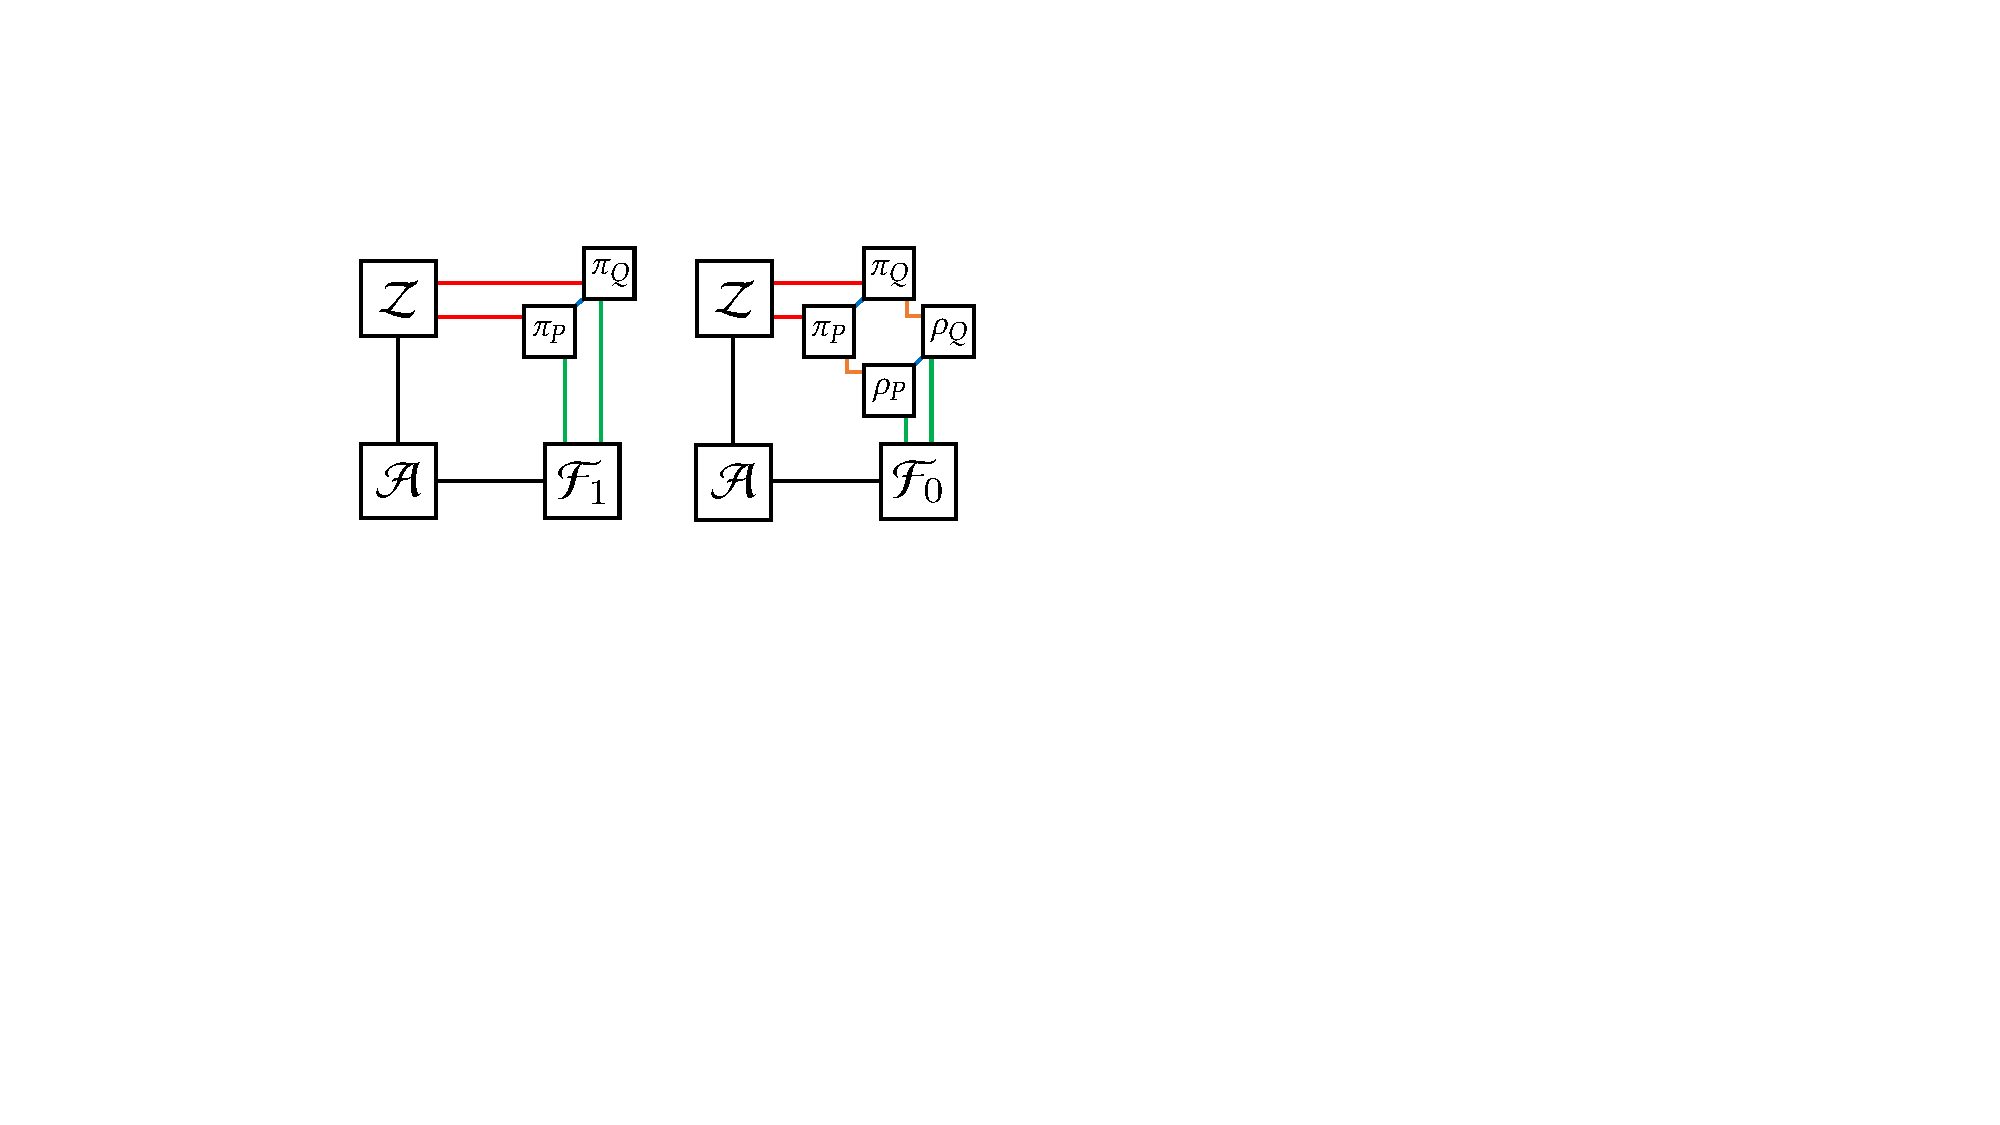
\includegraphics[width=0.85\linewidth]{graphics/protocol-composition}
  \caption{Protocol composition diagram.}
  \label{fig:protocol-composition}
\end{figure}

As a first usage of SaUCy, work through the development of a composition
operator, and give a composition theorem explaining its use.

\todo{Explain more the importance of composition operators}

Essentially, our operator is the notion of UC-realizes. We can now state useful
composition operators, simplifying lemmas, and notation. For brevity, we pack
several notions from UC into a single alternate definition: UC-realizes.

\begin{definition}[UC-realizes]
  Protocol $\pi$ with $\mc{F}_0$ realizes $\mc{F}_1$, written
  $\mc{F}_0 \yrightarrow{$\pi$} \mc{F}_1$, if for all environments $\mc{Z}$,
%  if $\keyword(\mc{Z}, \pi, \mc{F}_0, \mc{A}_{\mathbbm{1}})$, then
%  $|- \keyword{polyUC}(\mc{Z}, \pi_{\mathbbm{1}}, \mc{F}_1, \mc{S})$, and the
  %  following statistical indistinguishability relation holds

  \begin{mathpar}
    \Infer{realizes}
          {\forall~\mc{Z}.~ \keyword{Good}~\phi~\mc{F}_2~\mc{Z} =>\\\\
            \mathsf{execUC}\ \mc{Z}\ \pi\  \mc{F}_1\ 1_\mc{A} \le
            \mathsf{execUC}\ \mc{Z}\ \phi\ \mc{F}_2\ \mc{S}}
          {\mc{F}_0 \yrightarrow{$\pi$} \mc{F}_1}
  \end{mathpar}
\end{definition}

The idea is that the environment can arbitrarily and adaptively choose
inputs to the protocol $\phi$. So when we compose with an arbitrary other
protocol $\rho$, it is not any worse than what the environment could have
done. It essentially creates a proof obligation to ensure isolation of the
protocols.  While the intended use of universal composition is to replace an
ideal functionality with a protocol that securely realizes it, we define
protocol composition \todo{Let's just call it protocol composition, not
  universal composition. It's not really universal.} more generally in terms of
replacing one subroutine protocol with another. Given a protocol $\phi$, a protocol
$\rho$ that makes calls to $\phi$, \todo{instead of ``makes calls'', specify that the
  \textsf{toF} channel of $\rho$ is connected to the \textsf{fromZ} channel of
  $\phi$. } and a protocol $\pi$ that emulates $\phi$, then $\rho^{\phi -> \pi}$ is identical to
$\rho$ with the following modifications:
\begin{itemize}[leftmargin=*]
  \item When $\rho$ writes to $\phi$, $\rho^{\phi -> \pi}$ writes to $\pi$.
  \item When $\rho^{\phi -> \pi}$ receives a message from $\pi$, proceed as $\rho$ would when
    it receives the same message from $\phi$.
\end{itemize}

\begin{figure}
\lstinputlisting[style=myilc]{listings/compose.ilc}
\caption{Protocol composition operator.}
\label{fig:composition-operator}
\end{figure}

From UC-realizes, we can conclude the original UC formulation for arbitrary
composition:
\begin{theorem}[Composition Theorem]
  If $\mc{F}_0 \yrightarrow{$\pi$} \mc{F}_1$, then for all $\rho$ we
  have that $(\rho^{\pi}, \mc{F}_0)$ emulates $(\rho, \mc{F}_1)$.
\end{theorem}

\subsection{Instantiating UC Commitments}
\label{subsec:example}
We walk through the development of a UC instantiation for commitments.  UC
commitments can be instantiated with standard cryptographic assumptions, for
example the RSA problem.  Also rely on a ``trusted setup'', or common reference
string, essentially public parameters generated ahead of time (modeled as an
ideal functionality FCRS).

Instantiation proofs in UC follow a standard rhythm. We start with a security
definition as an ideal functionality, give the protocol, construct a simulator,
and finally complete the relational analysis on paper.  UC commitments are
reasoned to be secure assuming a common reference string is suitably generated.
To model the cryptography we extend ILC with additional syntax.

The functionality FCom has already been defined.
\todo{Recap the proof obligation}

\paragraph{Extending ILC with cryptographic primitives.}
\todo{Still lots of changes to make here.} UC Commitments are realized from
cryptographic primitives, such as pseudorandom trapdoor permutations. This
requires us to extend the syntax. The semantics are written in terms of the
cryptographic objects themselves, and we still arrive at a computational
reduction for our security proof.

The new syntactic forms are \textsf{kgen}, \textsf{tdp}, \textsf{inv}, and
\textsf{hc} with the static and dynamic semantics shown in
Figure~\ref{fig:extended-ilc}. The key generation function \textsf{keygen}
generates, on input $1^n$ (security parameter), a random public key $v_{pk}$ and
a trapdoor $v_{td}$. The trapdoor permutation function \textsf{tdp} computes, on
input key $v_k$ and bitstring $v_{in}$, a bitstring $v_{out}$. The hardcore
predicate function \textsf{hc} generates, on input trapdoor permutation
$f_{v_k}$.

\begin{figure*}
  \begin{grammar}
    Expressions
    & $e$
        &$\bnfas$&
        $\eKGen{e} \bnfalt \eTdp{e_1}{e_2} \bnfalt \eHc{e}$
  \end{grammar}
  
  \judgbox{\Delta ; \Gamma |- e : A |> m}{~~Under $\Delta$ and $\Gamma$, expression~$e$ has
  intuitionistic type $A$ and mode $m$.}
  \begin{mathpar}
  \Infer{kgen}
  {\Delta ; \Gamma |- e : [\tyBit]}
  {\Delta; \Gamma |- \eKGen{e}: [\tyBit]}
  %
  \and
  %
  \Infer{eTdp}
  {\Delta_1; \Gamma |- e_1 : [\tyBit]\\
   \Delta_2; \Gamma |- e_2 : [\tyBit]}
  {\Delta_1, \Delta_2; \Gamma |- \eTdp{e_1}{e_2}: [\tyBit]}
  %
  \and
  %
  \Infer{hc}
  {\Delta; \Gamma |- e : \tyArr{[\tyBit]}{}{\tyArr{[\tyBit]}{}{[\tyBit]}}}
  {\Delta; \Gamma |- \eHc{e}: \tyBit}
  \end{mathpar}
  
  \judgbox{\Store_1 ; e_1 ---> \Store_2 ; e_2}{~~Under store $\Store_1$,
    expression~$e_1$ reduces to~$\Store_2 ; e_2$.}
  \begin{mathpar}
  \Infer{kgen}
  {\keyword{\textbf{Gen}}(n) = (v_{pk}, v_{td}) \\ v_{pk}, v_{td} \in \{0,1\}^n}
  { \Store ; \eKGen{n} ---> \Store ; (v_{pk}, v_{td})}
  \and
  \Infer{tdp}
  {\mathbf{f}_{v_k}(v_i) = v_o \\ \mathbf{f} \colon \{0,1\}^n -> \{0,1\}^n -> \{0,1\}^n}
  { \Store ; \eTdp{v_k}{v_i} ---> \Store ; v_o }
  \and
  \Infer{hc}
  {\keyword{\textbf{Hc}}(\mathbf{f}_{v_k}) = v \\ \keyword{\textbf{Hc}} \colon
  (\{0,1\}^n -> \{0,1\}^n) -> \{0, 1\}}
  { \Store ; \eHc{f_{v_k}} ---> \Store ; v}
  \end{mathpar}
%  \begin{mathpar}
%    G_{pk}(r) = (f^{(3n)}_{pk}(r), B(f^{(3n-1)}_{pk}(r)), \ldots, B(f_{pk}(r)), B(r))
%  \end{mathpar}
  \caption{ILC extended with trapdoor permutations.}
  \label{fig:extended-ilc}
\end{figure*}


\[ G_{pk}(r) = \big(f_{pk}^{(3n)}(r), B(f_{pk}^{(3n-1)}(r)), \ldots, B(f_{pk}(r)), B(r)\big)\]

\lstinputlisting[style=myilc]{listings/prg.ilc}

\begin{algorithm}
\SetAlgorithmName{Protocol}{protocol}{List of Protocols}
\DontPrintSemicolon

\SetKwBlock{Parameters}{\textnormal{\textsf{Public strings}:}}{}
\Parameters{
  $\sigma$: Random string in $\{0,1\}^{4n}$\;
  ${pk}_0, {pk}_1$: Keys for generator $G_{k} \colon \{0,1\}^n \to \{0,1\}^{4n}$
}\smallskip
\SetKwBlock{Commit}{\textnormal{\textsf{Commit}($b$):}}{}
\Commit{
  $r \leftarrow \{0, 1\}^n$\;
  $x \coloneqq G_{{pk}_b}(r)$\;
  if $b=1$ then $x \coloneqq x \oplus \sigma$\;
  Send $(\mathsf{Commit}, x)$ to receiver.\;
  Upon receiving $(\mathsf{Commit}, x)$ from $A$, $B$ outputs $(\mathsf{Receipt})$.
}\smallskip

\SetKwBlock{Decommit}{\textnormal{\textsf{Decommit}($x$):}}{}
\Decommit{
  Send $(b, r)$ to receiver.\;
  Receiver checks $x = G_{{pk}_b}(r)$ for $b = 0$, or $x = G_{{pk}_b}(r) \oplus \sigma$
  for $b = 1$. If verification succeeds, then $B$ outputs $(\mathsf{Open}, b)$.
}
\caption{Universally Composable Commitment}
\label{alg:com}
\end{algorithm}

\begin{figure}
\lstinputlisting[style=myilc]{listings/ucc.ilc}
\caption{Universally composable commitment in ILC.}
\label{fig:ucc}
\end{figure}

\paragraph{Commitment Protocol.}
We defer the protocol to the appendix.

\paragraph{Defining the simulator.}

\paragraph{Relational argument.}

\subsection{Reentrancy in SaUCy}
\label{subsec:reentrancy}

The cryptography community has recently identified several subtleties in defining UC ideal functionalities that relate to ``reentrancy'' and scheduling of concurrent code;
as a consequence, many functionalities in the literature turn out to be ill-defined~\cite{camenisch2016universal}.
This subtle definitional issue, although important for the well-foundedness of security claims,
is not ``cryptographic'' in nature, and is better addressed from the PL viewpoint.
To illustrate, consider the following fragment of (untyped) ILC syntax, which allows an adversary to control the delivery schedule of messages from $P$ to $Q$ (an asynchronous channel):
\lstinputlisting[style=myilc]{listings/reentrant.ilc}
After receiving input from party $P$, it
notifies the adversary, then forks a background thread to wait for \textsf{OK} before
delivering the message.
This introduces a race condition: suppose input message $m_1$ is sent by $P$, but then the adversary $\mathcal A$, before sending \textsf{OK}, instead returns control to $\mathcal Z$, which passes $P$ a second input $m_2$. Now there are two queued messages; which one gets delivered first when the adversary sends \textsf{OK}?

To resolve this paradox, notice that fragment is untypeable in ILC.
The race condition occurs because of duplication of the read channel \textsf{frA}.
Since \textsf{frA} is linear in the function body, the function would not be typeable as intuitionistic as required by the \textsf{loop} construct.
Camenisch et al.~\cite{camenisch2016universal} identified several strategies for resolving this problem in UC, which in turn are expressible ILC. One approach is to make the process explicitly sequential, such that the arrival of a second message before the first is delivered causes execution to get stuck:
\lstinputlisting[style=myilc]{listings/reentrant-seq.ilc}
An alternative is to discard such messages arriving out of order, returning them to sender; this can be expressed in ILC using the external choice operator:
operator,
\lstinputlisting[style=myilc]{listings/reentrant-ignore.ilc}
